\section{Hyperbolic geometry}

It is the goal of this section to introduce a general method relying on the concepts of 2-dimensional hyperbolic geometry for the construction of fundamental regions with respect to the action of $\PSL{\Z}$ and its subgroups on $\EU$. Note that this method is applicable just as well in the more general context of \emph{discontinuous groups} acting on $\EC$ -- see \Lehner{}. 

\index{Hyperbolic geometry}
Plane (\ie 2-dimensional) hyperbolic geometry is obtained from 2-dimensional Euclidean geometry by replacing the parallel postulate by the following axiom: 
\begin{enumerate}[(A)]
\item
\emph{Let $P$ be a point and $L$ be a line on the (hyperbolic) plane, such that $L$ does not pass through $P$. Then there is more than one line $L^\prime$ passing through $P$ which does not meet $L$.}
\end{enumerate}

\index{Poincar{\'e}!half-plane model}
\index{Poincar{\'e}!disk model}
There are various models for hyperbolic geometry. For our purposes, the \emph{\Poincare{} half-plane model} and the $\emph{\Poincare{} disk model}$, which respectively identify the hyperbolic plane with the upper half-plane of $\C_\infty$ and the unit disk $\mathbb{D} \subseteq \C$, are most important. It is worth noting that there is a direct relation between these two models which is established through any M�bius transformation which maps the upper half-plane to the unit disk (or vice-versa).


\subsection{Normal polygons and fundamental regions}

%Vonroi diagram

\begin{figure}
\centering
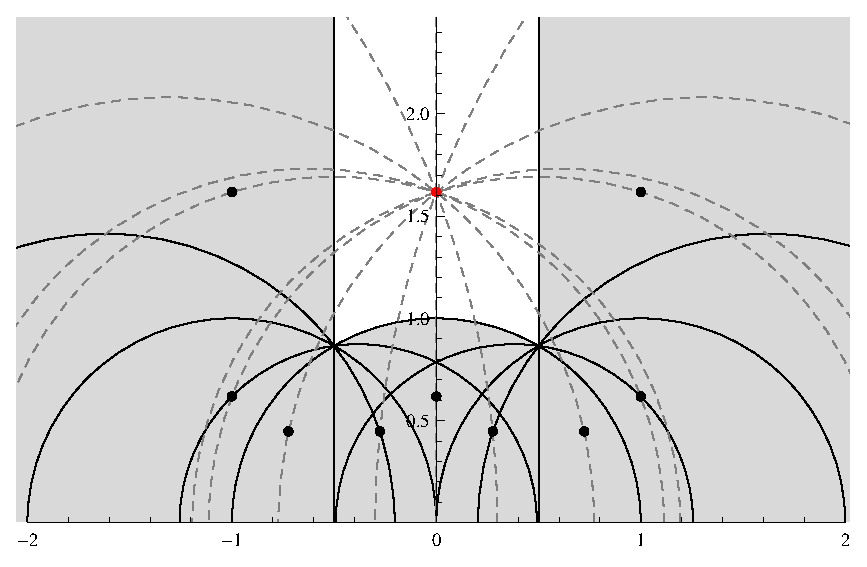
\includegraphics[width=\textwidth]{figures/normpoly-fundom-1}
\caption[The fundamental region $\FunDom$ as normal polygon]{The fundamental region $\FunDom$ can alternatively obtained by constructing the normal polygon with respect to a point $z$ on the imaginary axis with $\Im{z} > 1$. Above the point $z = \phi \ii$ (red) has been chosen, where $\phi = \frac{\sqrt{5}+1}{2}$ denotes the golden ratio.}
\label{fig_NormalPolyFunDom}
\end{figure}

\begin{figure}
\centering
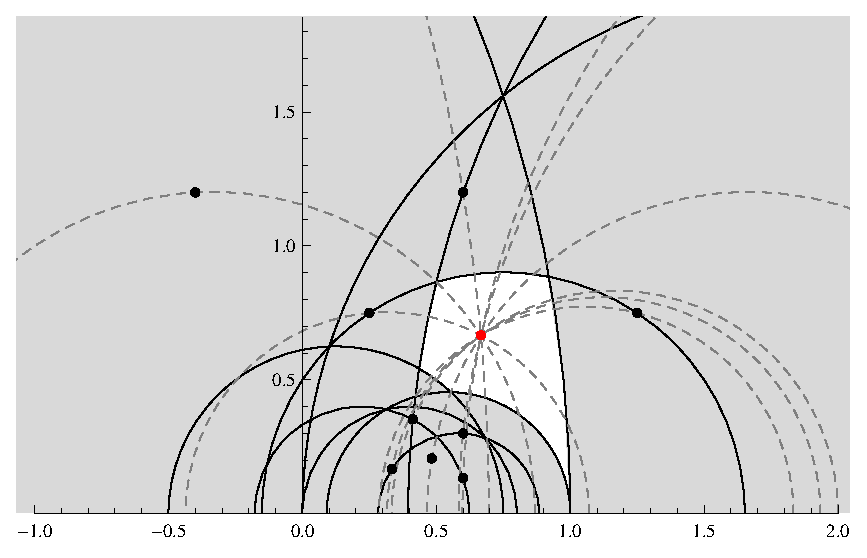
\includegraphics[width=\textwidth]{figures/normpoly-fundom-2}
\caption[An alternative fundamental region for $\PSL{\Z}$]{An alternative fundamental region for the action of $\PSL{\Z}$ on $\EU$. It is obtained by constructing the normal polygon for the point $\frac{2}{3}(1+\ii)$.}
\label{fig_AltNormalPolyFunDom}
\end{figure}

\begin{figure}
\centering
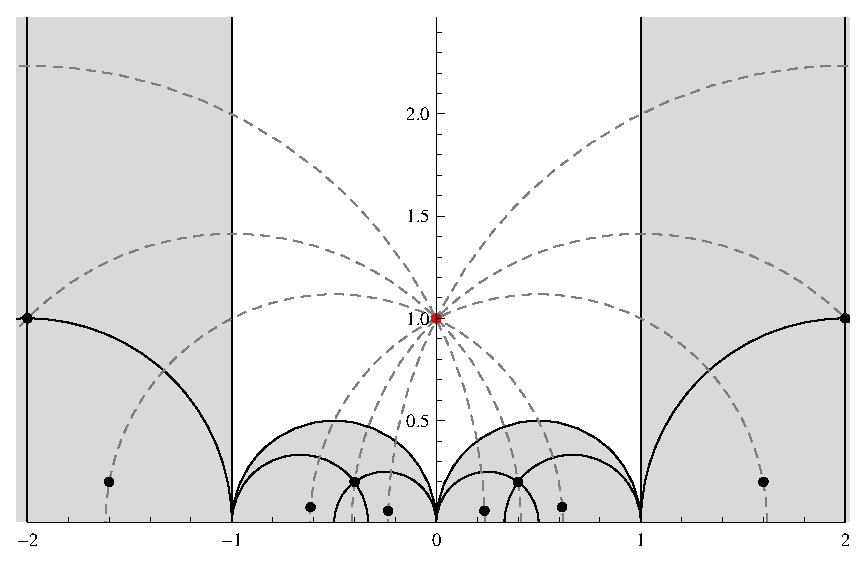
\includegraphics[width=\textwidth]{figures/normpoly-gamma2-1}
\caption[A fundamental region $\Gamma(2)$]{A fundamental region for the subgroup $\Gamma(2) \le \PSL{\Z}$. It is given by the normal polygon constructed with respect to the point $\ii$.}
\label{fig_Gamma2NormalPoly}
\end{figure}
